%%% -- -*- fill-column: 100; -*-

%% Include the preamble at choice during processing.
\documentclass[a4paper,10pt]{report}

%% This document is processed in an isolated clean folder at the same level
\makeatletter
\def\input@path{{../tex/}}
\makeatother

%% Page settings
%%% \usepackage[margin=0.5in,nomarginpar]{geometry}

%%% Bibliography system setup using biblatex
\usepackage[
    backend=biber,
    style=alphabetic,
]{biblatex}
\addbibresource{../tex/Biblio.bib}

%% Packages
\usepackage[utf8]{inputenc}
\usepackage{hyperref}
\usepackage{fvextra}
\usepackage{csquotes}
\usepackage{xcolor}
\usepackage{minted}
\usepackage{amsfonts}
\usepackage{amsmath}
\usepackage{graphicx}
\usepackage{enumitem}

%% Formatting

\renewcommand{\mkbegdispquote}[2]{\itshape}

%% Required Literate Haskell (lhs) macros (code, spec)
%%% include common lhs formatting
\input{lhsfmt.tex}
%%% for code
\newminted[code]{haskell}{}
\newminted[spec]{haskell}{}

%% Other macros
\long\def\ignore#1{} % for ignoring code
\newcommand{\eg}{\textit{e}.\textit{g}.}
\newcommand{\ie}{\textit{i}.\textit{e}.}
\newcommand{\etal}{\textit{et al}.}

%% Used Unicodes in code
\DeclareUnicodeCharacter{03BD}{$\nu$}
\DeclareUnicodeCharacter{2205}{$\emptyset$}
\DeclareUnicodeCharacter{2295}{$\oplus$}
\DeclareUnicodeCharacter{27E6}{$[\![$}
\DeclareUnicodeCharacter{27E7}{$]\!]$}
\DeclareUnicodeCharacter{1D4DC}{$\mathcal{M}$}


\begin{document}

\title{Denotational Semantics of General Payment Primitives, and Its Payment System}

\author{\\
    Miao, ZhiCheng\\
    Co-founder, Superfluid Finance\\
    miao@superfluid.finance
}

%%%%%%%%%%%%%%%%%%%%%%%%%%%%%%%%%%%%%%%%%%%%%%%%%%%%%%%%%%%%%%%%%%%%%%%%%%%%%%%%%%%%%%%%%%%%%%%%%%%%
%% Title Page
%%%%%%%%%%%%%%%%%%%%%%%%%%%%%%%%%%%%%%%%%%%%%%%%%%%%%%%%%%%%%%%%%%%%%%%%%%%%%%%%%%%%%%%%%%%%%%%%%%%%

\maketitle

\begin{abstract}
Payment systems in information age are still largely modeled after their analog predecessors. While
electronic money payment systems do utilize computing technology and Internet, this paper presents a
case that a true modernization can be reached by (a) making payments happening continuously over
time, (b) involving more than two parties in a payment if necessary, (c) having compositional
financial contracts.

This paper first explores the foundation of modern payment system, which consists of a money
distribution model, payment primitives, payment execution systems of financial contracts and
different forms of money mediums. Then the paper uses \textit{denotational semantics} to formally
define payment primitives for modern payment system. Lastly, this paper also includes an overview
of \textit{Superfluid protocol}, a reference implementation of the payment primitives and its
payment system.

This paper includes literate Haskell code that compiles as the constructive artifact for the formal
specifications.

This paper is also the first one in the series of yellowpapers about modern payment system dubbed
``semantic money''.

\end{abstract}

\part*{Introduction}
%%%%%%%%%%%%%%%%%%%%

It should be fair to say, every aspect of money is controversial: the nature of money, the value of
money, money and banking, and monetary reconstruction. Two major schools of thoughts about theory of
money are the \textit{Austrian school} (\cite{von2013theory}) and the \textit{Chicago school}
(\cite{friedman1989quantity}). That is before the appearance of Internet-era version of monetary
reconstruction, broadly defined as cryptocurrency, which challenges theories of money further and
demands their updates (\cite{ammous2018can} \cite{hardle2020understanding}).

This yellow paper does not intend to address these controversies, instead it focuses on the function
of money. According to Von Mises:

\begin{displayquote}
The function of money is to facilitate the business of the market by acting as a common medium of
exchange. \footfullcite[][Chapter One, Chapter I, § 1, p1]{von2013theory}
\end{displayquote}

How do different forms of money perform this function, especially in the information age, when
electronic forms of money are increasingly used?

This paper adds a new controversy to money, that is to present a foundation of what constitutes of
a \textit{modern payment system} and a set of \textit{payment primitives} for the system, in order
to challenge the preconceived notions of how money can perform its function of medium of exchange.

In part \ref{part:foundation}, we shall first explore the foundation. Here we present a formal
definition of payment system and its components. We then select a few relevant approaches used in
computer science useful for modeling and defining formal specification for the payment system.

One of the approaches is \textit{denotational semantics}, which is used in part \ref{part:gpp} of
the paper to define the \textit{general payment primitives}. Along with the denotational semantics,
a restatement\footnote{It is a borrowed term from common law: ``restatement of the law''. In our
case, the denotative mathematical laws.} of it in \textit{Haskell programming language}
(\cite{hudak1992report} \cite{jones2003haskell} \cite{marlow2010haskell}) is also included.

In part \ref{part:sf}, a reference implementation of the general payment primitives and its payment
system called \textit{Superfluid Protocol} is introduced with an overview of it.

Notes on possible further investigations are also included in the end of the paper.

%%%%%%%%%%%%%%%%%%%%%%%%%%%%%%%%%%%%%%%%%%%%%%%%%%%%%%%%%%%%%%%%%%%%%%%%%%%%%%%%%%%%%%%%%%%%%%%%%%%%
\part{Foundation}\label{part:foundation}
%%%%%%%%%%%%%%%%%%%%%%%%%%%%%%%%%%%%%%%%%%%%%%%%%%%%%%%%%%%%%%%%%%%%%%%%%%%%%%%%%%%%%%%%%%%%%%%%%%%%

%%%%%%%%%%%%%%%%%%%%%%%%
\section{Payment System}
%%%%%%%%%%%%%%%%%%%%%%%%

Here we present a definition of payment system and its components.

\paragraph{Payment system}

It is solely defined by these components:

\begin{itemize}
    \item \textit{money distribution} models how monetary value is distributed amongst
bearers \footnote{(Banking \& Finance) a person who presents a note or bill for payment. - Collins
English Dictionary},

    \item \textit{payment primitives} updates money distribution,

    \item \textit{payment execution environment} performs payment primitives encoded
    in \textit{financial contracts},

    \item and \textit{forms of money medium} are the ``user interfaces'' of money for the bearers.
\end{itemize}

\paragraph{Modernization}

For its modern upgrade, the system should also have these properties:

\begin{itemize}
    \item Money can be distributed continuously over time, as opposed to be in discrete chunks.

    \item Payment primitives can involve more than two parties, as opposed to be only for a sender
and a receiver.

    \item Financial system should be compositional.
\end{itemize}

\subsection{Money Distribution}
%%%%%%%%%%%%%%%%%%%%%%%%%%%%%%%

A representation of money and its distribution proposed in ``a unifying theory''
from \citeauthor{buldas2021unifying} involves the following components:

\begin{itemize}
    \item U is the set of monetary units.

    \item $\nu : U \rightarrow \mathbb{N}$ is the value function defining the value $\nu(u)$ of
every value unit u. The set $\mathbb{N}$ is the set of all natural numbers, but instead, we can use
any set of numerals that is totally ordered (\eg\ integers, real numbers).

    \item $\beta : U \rightarrow \mathcal{B}$ is the bearer function defining the bearer $\beta(u)$
of a unit. The set $\mathcal{B}$ is the set of possible bearers. The bearer is usually a legal
construction defining any type of legal entity, such as a person, a family, a company, a state
institution, etc.
\end{itemize}

This discrete nature of this money distribution model is schematically depicted
in figure \ref{fig:discrete-md}.

\begin{figure}[h]
    \centering
    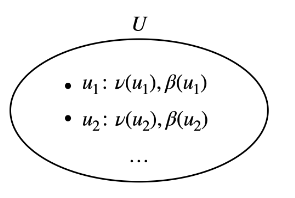
\includegraphics[width=0.5\textwidth]{../assets/discrete-money-distribution.png}
    \caption{Schematic representation of discrete money distribution}
    \label{fig:discrete-md}
\end{figure}

\subsubsection{Adding Context $\gamma$}

But the discrete nature of the model does not provide the necessary element for us to add the
desired properties to the payment system. Here we propose a modification that involves the usage
of \textit{context ($\gamma$)}:

\begin{figure}[h]
    \centering
    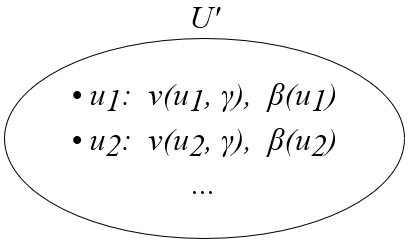
\includegraphics[width=0.5\textwidth]{../assets/money-distribution-with-ctx.png}
    \caption{Schematic representation of money distribution with context}
    \label{fig:md-with-ctx}
\end{figure}

Note that in this model, context can be updated independently while value functions of the same
money distribution can produce different monetary values.

\paragraph{Components of Context}

Here are some possible components of context, and how they work:

\begin{itemize}
    \item If time (t) is included the context, then monetary value of each monetary unit can vary
continuously over time. Time is part of the physical reality, hence not changeable by the actors in
the payment system.

    \item Any subset of monetary units can also have their value functions depending on the same
information in context. This could enable payment primitives that involve many parties. This set of
information in context is referred to as \textit{ctx :: SharedContext}, they can be changed over
time by the actors in the payment system.
\end{itemize}

For the purpose of this paper, the model of context is: $\gamma = t \times ctx$.

\subsubsection{Haskell Code Conventions Used}

Before the first time in this paper listing specification in Haskell, here are some highlights of
conventions in the style of the code used.

\paragraph{Language Extensions}

The specification is written in Haskell with \textit{GHC2021 language set}\footnote{The complete set
of the extensions is enumerated in
\url{https://downloads.haskell.org/ghc/latest/docs/users_guide/exts/control.html\#extension-GHC2021}.}.

Other notable extensions used in the paper are: $FunctionalDependencies$, $TypeFamilies$,
$TypeFamilyDependencies$, $GADTs$.

\paragraph{Indexed Types and Type Equality}

In order to make the specification free of specific choices of core data types in
implementation, \textit{FunctionalDependencies}, \textit{TypeFamilies}
and \textit{TypeFamilyDependencies} are extensively used. As a consequence, the type signature can
look very cluttered. In order to address that, type quality operator $(\sim)$ is also used. Here is
an example snippets:

\begin{code}
    type (~) :: forall k. k -> k -> Constraint

    monetaryValue :: ( mv  ~ MD_MVAL md
                     , mu  ~ MD_MU md
                     , ctx ~ MD_CTX md
                     )
                  => md -> (mu, ctx) -> mv
\end{code}

The otherwise tedious type family synonyms ``\mintinline{haskell}{MD_XYZ md}'' are rewritten with $mv$
$mu$ $ctx$ with the help of $(\sim)$ operator.

\subsubsection{Haskell Definition Of Money Distribution}

\input{MoneyDistribution.lhs.tex}

\subsection{Payment Primitives}
%%%%%%%%%%%%%%%%%%%%%%%%%%%%%%%

A payment primitive is a data type with a generator function that produces payment primitive from
the shared context $ctx$, primitive specific argument $args$ and timestamp $t$, along with an update
of the shared context. Type signature \ref{eq:genPrim} is for the generator of payment
primitive \textit{a}:

\begin{equation}\label{eq:genPrim}
    genPrim_a :: ctx \rightarrow args_a \rightarrow t \rightarrow prim \times ctx
\end{equation}

Payment primitive data then can be used to create a delta update of money
distribution\footnote{Specifically being monoidal, that is in short a set that has associative
binary operation and an identity element. See https://ncatlab.org/nlab/show/monoid.}:

\begin{equation}
    runPrim :: prim \rightarrow md
\end{equation}

Loosely speaking, it is considered a primitive, if it can not be broken down into other existing
primitives which result in the same money distribution; additionally primitives should be the only
constructs in a payment system that can update money distribution.

Updates are \textit{monoidal}, so that they can be incremental and their parallel executions can be
modeled.

The most known primitive is instant transfer of monetary value between one monetary unit to
another. The introduction of context enables more primitives to be defined, and this will be
discussed in part \ref{part:gpp}.

\subsection{Payment Execution Environment}
%%%%%%%%%%%%%%%%%%%%%%%%%%%%%%%%%%%%%%%%%%

The purpose of a payment execution environment is to perform the actual payment primitives, where
their computation interface, parallel evaluation strategies and payment system solvency are defined.

It is out of scope for this paper to survey in-depth the problem space of the operational semantics
of payment execution environments. Nonetheless, a simplified model and some potential extensions to
it is discussed briefly to place payment primitives in the big picture.

\subsubsection{Composing Financial Contracts}

\input{FinancialContract.lhs.tex}

\subsubsection{Simplified Execution Environment Models}

\input{PaymentExecutionEnvironment.lhs.tex}

\subsection{Payment System Solvency}

While money distribution does not assign meaning to the range of monetary values, in real world
applications, negative values can have special meanings. In the following analysis, we call any
money unit that has a negative monetary value \textit{insolvent}.

The detailed analysis of these solvency models are out of scope for this paper.

\paragraph{Buffer Based Solvency Treatment}

In a nondeterministic execution environment, we cannot determine when any financial contract will
actually be executed. That means, there is always a chance a monetary unit could reach negative
monetary value.

To mitigate this uncertainty, a concept called \textit{buffer} is introduced. A buffer has a
monetary value which is set aside in a solvency conditional financial contract, such that if a
solvency condition arises, the buffer maybe drawn to cover the loss introduced by the
nondeterministic timing of the execution.

\paragraph{Deterministic Solvency Treatment}

Since \textit{fcNext} returns what is the next financial contract executable at a specific time,
this deterministic property eliminates the need for the buffer.

On the other hand, it introduces a different type of systemic risk, that is a kind of
denial-of-service. It is due to that the complexity of $fcUpdate$ is $O(log(n))$, the system may not
be able to advance its system time until all next executable contracts are executed.

\subsection{Money Mediums}
%%%%%%%%%%%%%%%%%%%%%%%%%%%%%%%%

\begin{displayquote}
A useful observation about existing money schemes is that they all have some kind of monetary units
that are physical or digital representations of money. Examples are bills, coins, bank accounts,
Bitcoin UTXOs, etc. \footfullcite[][P3]{buldas2021unifying}
\end{displayquote}

We call them money mediums, and we further separate them into two big groups:

\begin{itemize}
    \item \textit{Token and its Accounts} - \eg\ bank currency accounts. Each token is its own
centralized execution environment, bearers access their monetary value through their accounts, and
execute financial contracts through the token.

    \item \textit{Note} - \eg\ federal reserve notes, bills, coins and Bitcoin UTXOs, etc. The
execution environment is independent of the notes, but it needs notes to complete the execution of
financial contracts.
\end{itemize}

One of the main differences is from the ``user interface'' perspective. A bearer expects to keep
many notes at hand, while maybe only needs a few accounts for each token. Also it is up to bearers
to keep track of all their notes, while token can keep track of most of the states for bearers;
hence notes are more decentralized and tokens are more centralized. Some also argue note-like model
is better for complex concurrent and distributed computing environment
\footfullcite[][P2]{chakravarty2020extended}.

\subsubsection{Haskell Definition Of Money Mediums}

\input{MoneyMedium.lhs.tex}

%%%%%%%%%%%%%%%%%%%%%%%%%%%%%
\section{Relevant Approaches}
%%%%%%%%%%%%%%%%%%%%%%%%%%%%%

The focus of this paper is to formally define a set of payment primitives that modernize our payment
systems. To prevent reinventing wheels, it is relevant to discuss first some approaches in computer
science that are believed to help tackling this challenge.

\subsection{Functional Reactive Programming}
%%%%%%%%%%%%%%%%%%%%%%%%%%%%%%%%%%%%%%%%%%%%

Recall that we want our modern payment system to handle money distribution continuously over time,
and its financial contracts compositional. A very closely related software design paradigm best
known to address those needs is \textit{functional reactive programming (FRP)}.  It was first
introduced by Conal Elliott \& Paul Hudak in solving multimedia animations
(\cite{elliott1997functional}). Later on, Hudak also worked on \cite{hudak2002arrows} and
\cite{wan2000functional} making FRP a more general framework for programming hybrid system with
continuous behaviors in a high-level, declarative manner.

After FRP got more adoption, it evolved to some variations that support discrete semantics, and some
variations better suited for interactive systems. In this paper we will stick to and revisit the
basic constructs of the original formulation used in \cite{elliott1997functional} where we will draw
inspirations from.

\paragraph{Temporal Modeling and Behaviors}

Values that vary over continuous time are called \textit{behaviors}. They are first-class values,
and are built up compositionally. That is what we want in modern payment system also. The semantic
function of $\alpha$-behaviors produces the value of type $\alpha$ of a behavior at a given time:

\begin{equation}
    at : Behavior_{\alpha} \rightarrow Time \rightarrow \alpha
\end{equation}

\paragraph{Event Modeling}

Like behaviors, \textit{events} are first-class values too. The semantic function of $\alpha$-event
describes the time and information associated with an \textit{occurrence} of the event:

\begin{equation}
    occ : Event_{\alpha} \rightarrow Time \times \alpha
\end{equation}

In modern payment system, the payment primitives executed in payment execution environments are
one type of events. More types of events can be read from the original paper \footfullcite[][section
2.3 Semantics of Events]{elliott1997functional}.

\paragraph{Reactivity}

They key to modeling the payment execution environment using FRP is the \textit{reactivity}, which
makes behaviors reactive. Specifically, the behavior \textit{b untilB e} exhibits b's behavior
until \textit{e} occurs, and then swiches to a new behavior encoded in \textit{e}:

\begin{equation}
    \begin{split}
    &untilB : Behavior_{\alpha} \rightarrow Event_{Behavior_{\alpha}} \rightarrow Behavior_{\alpha} \\
    &at\ [\![b\ until\ B]\!]\ t = if\ t\ \leq\ t_{e}\ then\ at\ [\![b]\!]\ t\ else\ at\ [\![b']\!]\ t \\
    &\qquad where (t_e, b') = occ[\![e]\!]
    \end{split}
\end{equation}

Note that $[\![.]\!]$ is the denotational semantics notation to be introduced later.

In the context of modern payment system, the occurrences of payment primitives (events) change the
behaviors of monetary units in how much monetary values it has over continuous. The building blocks
of the financial contracts should be about modeling these events and their reactivity declaratively.

\subsection{Denotational Semantics}
%%%%%%%%%%%%%%%%%%%%%%%%%%%%%%%%%%%

We also want a formal and precise specification of payment primitives. The title of the paper
includes \textit{denotational semantics}: ``it is a \textit{compositional} style for precisely
specifying the meanings of languages, invented by Christopher Strachey and Dana Scott in the 1960s
(\cite{scott1971toward})'', and Conal Elliott proposed that denotational semantics can also be
applied to \textit{data types within a programming language}
\footfullcite[][section 2, denotational semantics and data types]{Elliott2009-type-class-morphisms-TR}.

To create denotational semantics for each syntactic category $\mathcal{C}$, we should specify:

\begin{itemize}
\item a mathematical model $[\![\mathcal{C}]\!]$ of meanings, and
\item a semantic function $[\![.]\!]_{\mathcal{C}} :: \mathcal{C} \rightarrow [\![\mathcal{C}]\!]$.
\end{itemize}

The syntactic category we are interested in is \textit{payment primitives}, which we should treat
them as FRP-style \textit{Behavior} data types. In the following chapters, it is also unambiguously
referred to in short as $[\![.]\!]$. Various $[\![.]\!]$ must be compositional, \ie\ must be defined
by structural recursion.

It is important to note that our purpose of using the denotational semantics is to give precise
meaning to payment primitives, independent of its implementation (which deals with performance,
optimization, side effects, etc.). We will spend the part \ref{part:gpp} exploring the denotational
semantics for general payment primitives in modern payment system.

%%%%%%%%%%%%%%%%%%%%%%%%%%%%%%%%%%%%%%%%%%%%%%%%%%%%%%%%%%%%%%%%%%%%%%%%%%%%%%%%%%%%%%%%%%%%%%%%%%%%
\part{General Payment Primitives}\label{part:gpp}
%%%%%%%%%%%%%%%%%%%%%%%%%%%%%%%%%%%%%%%%%%%%%%%%%%%%%%%%%%%%%%%%%%%%%%%%%%%%%%%%%%%%%%%%%%%%%%%%%%%%

The set of payment primitives supported in a payment system is general, if (a) monetary value of
each monetary unit can vary continuously over time (b) monetary values can logically be shifted
between two or more monetary units.

The extent of the generality of each payment system may vary. This paper introduces a set of payment
primitives that is general and serves as a starting point for the readers to explore the space of
modern payment system.

The specifications will be formally defined using denotational semantics, along with a restatement
in Haskell also applied as a constructive artifact friendly to computer environment\footnote{One may
argue for a restatement in \textit{Agda} instead, for it has a richer dependently-type system for
desirable constructive proofs. This matter will be dealt in the ``future investigations'' section of
this paper.}.

%%%%%%%%%%%%%%%%%%%%%%%%%%%%%%%%
\section{Denotational Semantics}
%%%%%%%%%%%%%%%%%%%%%%%%%%%%%%%%

Here is the convention for symbols used in the formulas:

\begin{itemize}
\item \textbf{M} is the \textit{model for money distribution}.
\item \textbf{m} is for \textit{money distributions}.
\item \textbf{U} is the \textit{set of all money units} in money distribution.
\item \textbf{u} is for \textit{monetary units}.
\item $\boldsymbol{\nu}$ is for \textit{monetary values}.
\item \textbf{t} is for \textit{time}.
\end{itemize}

\subsection{$\mathcal{M}$ - Syntax for Money Distribution}

Recall the definition of payment system previously, money distribution sits in the core of the
system, and that is the syntactic category $\mathcal{M}$ we will be dealing with:

\begin{itemize}
    \item The meaning of the mathematical \textit{model} $[\![\mathcal{M}]\!]$ is money distribution.

    \item Semantic function $[\![.]\!] :: \mathcal{M} \rightarrow [\![\mathcal{M}]\!] $ evaluates
the expression of money distribution, payment primitives, etc.
\end{itemize}

\subsection{Money Distribution}
%%%%%%%%%%%%%%%%%%%%%%%%%%%%%%%

\paragraph{Model}

This is the model for money distribution.

\begin{equation}\label{md_model}
    \begin{split}
        [\![M\ u\ t\ \nu]\!] &= u \rightarrow t \rightarrow \nu \\
        [\![.]\!] &= M\ u\ t\ \nu \rightarrow (u \rightarrow t \rightarrow \nu) \\
    \end{split}
\end{equation}

\paragraph{Monoidal}

With this model, $\mathcal{M}$ is also monoidal, hence compositional.

\begin{equation}
    \begin{split}
        [\![\emptyset]\!] &= \lambda u \rightarrow \lambda t\ \rightarrow \emptyset \\
        [\![m_a \oplus m_b]\!] &= \lambda u \rightarrow \lambda t\ \rightarrow
            [\![m_a]\!]\ u\ t\ +\ [\![m_b]\!]\ u\ t \\
    \end{split}
\end{equation}

Knowing that function application category $a \rightarrow b$ is also monoidal:

\begin{equation}
    \begin{split}
        \emptyset &= \lambda a \rightarrow \emptyset \\
        f \oplus g &= \lambda a \rightarrow f\ a \oplus g\ a \\
    \end{split}
\end{equation}

With some substitutions, we get the desired \textit{monoid homomorphism} property for $\mathcal{M}$.

\begin{equation}
    \begin{split}
        [\![\emptyset]\!] &= \emptyset \\
        [\![m_a \oplus m_b]\!] &= [\![m_a]\!] \oplus [\![m_b]\!] \\
    \end{split}
\end{equation}

\subsection{Payment Primitives}
%%%%%%%%%%%%%%%%%%%%%%%%%%%%%%%

A payment primitive \textit{prim} is a model that produces a monoidal money distribution,
semantically representing an ``update'' to a money distribution:

\begin{equation}
    [\![prim]\!] = [\![\Delta\ m]\!]
\end{equation}

\paragraph{Law of Conservation of Value}

First of all, money distribution must obey the \textit{law of conservation of value}:

\begin{equation}
    \forall t \in \mathbb{R} {\displaystyle \sum_{u \in U} [\![m]\!]\ u\ t = 0}
\end{equation}

That is to say, at any given time, the sum of monetary value of all monetary units shall always
equal to zero. Zero is used to keep the semantical meaning of payment system simple and elegant. In
its applications, a payment system may use some special monetary unit accounting negative monetary
values to accommodate concepts such as mining, minting, money printing, etc.

\paragraph{Restricted Money Distribution}

To come up with such lawful money distribution, we can divide and conquer. In a payment system, if
we restrict that only payment primitives can provide ``updates'' to its money distribution, so that
a money distribution is only a result of a sequence of payment primitive updates; then we can have
these axioms as the basis for the proof.

\paragraph{Axiom A of Restricted Money Distributions}

First we must impose the law of conservation of value on payment primitives as an axiom, in order to
prove inductively that such restricted money distribution satisfies the law of conservation of value
too.

\begin{equation}
    \begin{split}
        &\textit{law of conservation of value for payment primitives} \\
        &\forall t \in \mathbb{R} ({\displaystyle \sum_{u \in U} [\![prim]\!]\ u\ t = 0}) \\
    \end{split}
\end{equation}

\paragraph{Axiom B of Restricted Money Distributions}

\begin{equation}
    \begin{split}
        &\textit{money distribution consists of updates from payment primitives} \\
        &[\![m]\!] = [\![prim_1]\!] \oplus [\![prim_2]\!] \oplus [\![prim_3]\!] \oplus \dotsb
    \end{split}
\end{equation}

\paragraph{Proof of Restricted Money Distributions}

satisfying the law of conservation of value.

\begin{equation}
    \begin{split}
        &\textbf{In addition to the axioms, given:} \\
        \\
        &\textit{(base case with empty money distribution is trivial)} \\
        &\forall t \in \mathbb{R} {\displaystyle \sum_{u \in U} [\![\emptyset]\!]\ u\ t = 0} \\
        \\
        &\textit{(monoid homomorphism)} \\
        &{\displaystyle \sum_{u \in U} [\![prim_1 \oplus prim_2]\!]\ u\ t} =
          {\displaystyle \sum_{u \in U} [\![prim_2]\!]\ u\ t} \oplus
          {\displaystyle \sum_{u \in U} [\![prim_2]\!]\ u\ t} \\
        \\
        &\textbf{We have:} \\
        &\forall t \in \mathbb{R}. \\
        &{\displaystyle \sum_{u \in U} [\![m]\!]\ u\ t} \\
        &\textit{(applying Axiom B)} \\
        = &{\displaystyle \sum_{u \in U}
            ([\![prim_1]\!] \oplus
            [\![prim_2]\!] \oplus
            [\![prim_3]\!]\oplus \dotsb)
        }\ u\ t
        \\
        &\textit{(applying monoid homomorphism)} \\
        = &{\displaystyle \sum_{u \in U} [\![prim_1]\!]\ u\ t} \oplus
        {\displaystyle \sum_{u \in U} [\![prim_2]\!]\ u\ t} \oplus
        {\displaystyle \sum_{u \in U} [\![prim_3]\!]\ u\ t} \oplus \dotsb
        \\
        &\textit{(applying Axiom A)} \\
        =&\ 0
        \\
        \blacksquare
    \end{split}
\end{equation}

\subsection{One to One Payment Primitives}
%%%%%%%%%%%%%%%%%%%%%%%%%%%%%%%%%%%%%%%%%%

Here are the primitives involving a sender ($u_a$) and a receiver ($u_b$) (one to one payments).

\paragraph{Transfer}

Instant transferring of a fixed amount of monetary value $x$:

\begin{equation}
    \begin{split}
        [\![transfer\ u_a\ u_b\ x]\!] &=
        \lambda u \rightarrow \lambda t \rightarrow \\
        &\begin{cases}
            -x & (u_a = u) \\
             x & (u_b = u) \\
             0 & (otherwise)
        \end{cases}
    \end{split}
\end{equation}

\paragraph{(Constant) Flow}

Flowing of monetary value at a constant rate of $r$ at time $t'$:

\begin{equation}
    \begin{split}
        [\![flow\ u_a\ u_b\ r\ t']\!] &=
        \lambda u \rightarrow \lambda t \rightarrow \\
        &\begin{cases}
            -r \cdot (t - t') & (u_a = u) \\
             r \cdot (t - t') & (u_b = u) \\
                            0 & (otherwise)
        \end{cases}
    \end{split}
\end{equation}

\paragraph{Decaying Flow}

Another way monetary value could flow is through an exponential decay
function\footnote{\url{https://en.wikipedia.org/wiki/Exponential_decay}.}.

Symbolically, this process can be expressed by the following differential equation, where N is the
quantity and $\lambda$ is a positive rate called the exponential decay constant:

\begin{equation}
    {\displaystyle {\frac {dN}{dt}}=-\lambda N}
\end{equation}

The solution to this equation (see derivation below) is:

\begin{equation}
    {\displaystyle N(t)=N_{0}e^{-\lambda t}}
\end{equation}

But a more convenient semantics of it uses the parameter called ``distribution limit'' ($\theta$)
instead. In this formulation, a decaying flow distributes $\epsilon$ amount of monetary value at a
rate started at $\alpha$ and halving every time period of $\displaystyle \frac{ln(2)}{\lambda}$:

\begin{equation}
    \begin{split}
        [\![decayingFlow\ u_a\ u_b\ \theta\ \lambda\ t']\!] &=
        \lambda u \rightarrow \lambda t \rightarrow \\
        &\begin{cases}
             {\displaystyle  \alpha \cdot e^{-\lambda (t' - t)} - \theta} & (u_a = u) \\
             {\displaystyle -\alpha \cdot e^{-\lambda (t' - t)} + \theta} & (u_b = u) \\
             0 & (otherwise)
        \end{cases}
    \end{split}
\end{equation}

For the simplicity of the later discussion, this form of payment primitive is omitted.

\subsection{Index Abstraction}
%%%%%%%%%%%%%%%%%%%%%%%%%%%%%%

To make primitives support more than two parties, we introduce an abstraction called \textit{index}.

A \textit{index} (we use symbol $k$ for them) has a function $\rho$ which produces a real number for
each monetary unit:

\begin{equation}
    \rho\ k :: u \rightarrow \mathbb{R}
\end{equation}

To make it meaningful, it must satisfy the following law:

\begin{equation}
    \displaystyle \sum_{u \in U} \rho\ k\ u = 1
\end{equation}

Semantically, it represents a proportion of each money unit, and they must add up to 1.

\subsection{Indexed Primitives}

Let's generalize the one to one payment primitives using index abstraction. We use $I$ subscript for
the indexed versions of the primitives.

\paragraph{Indexed Transfer}

\begin{equation}
    \begin{split}
        [\![transfer_I\ k_a\ k_b\ x]\!] &=
        \lambda u \rightarrow \lambda t \rightarrow \\
        &-x \cdot \rho\ k_a\ u + x \cdot \rho\ k_b\ u
    \end{split}
\end{equation}

\paragraph{Indexed (Constant) Flow}

\begin{equation}
    \begin{split}
        [\![flow_I\ k_a\ k_b\ r\ t']\!] &=
        \lambda u \rightarrow \lambda t \rightarrow \\
        &-r \cdot (t - t') \cdot \rho\ k_a\ u + r \cdot (t - t') \cdot \rho\ k_b\ u
    \end{split}
\end{equation}

It should be straightforward to prove that they also satisfy the \textit{axiom A of restricted money
distribution} thanks to the law of the index.

\paragraph{Universal Index}

Now one to one payment primitives can be redefined using \textit{universal index} ($ku_{any}$):

\begin{equation}
    \rho\ ku_{a} = \lambda u \rightarrow if\ u\ =\ u_a\ then\ 1\ else\ 0
\end{equation}

It means that it is an index \textit{universally} available for each monetary unit, and its
proportion is always 1 for that monetary unit and 0 for all others.

\paragraph{Proportional Distribution Primitives}

A special case of the indexed primitives is to fix the sender side to be an \textit{universal
index}.

\subsection{Network Abstraction}

An even more general abstraction is to model participants involved a payment primitive
a \textit{network} (we use symbol $w$ for them).

It has the function $\rho$ as in \textit{index}, bnd it satisfies a different law:

\begin{equation}
    \displaystyle \sum_{u \in U} \rho\ w\ u = 0
\end{equation}

\subsection{Networked Primitives}

Let's generalize the basic payment primitives using network abstraction. We use $N$ subscript for
the indexed versions of the primitives.

\paragraph{Shift}

We rename $transfer$ to $shift$ for networked instant payment primitive:

\begin{equation}
    \begin{split}
        [\![shift_N\ w\ x]\!] &=
        \lambda u \rightarrow \lambda t \rightarrow x \cdot \rho\ w\ u
    \end{split}
\end{equation}

\paragraph{Networked (Constant) Flow}

\begin{equation}
    \begin{split}
        [\![flow_N\ w\ r\ t']\!] &=
        \lambda u \rightarrow \lambda t \rightarrow r \cdot (t - t') \cdot \rho\ w\ u
    \end{split}
\end{equation}

\subsection{Generality vs. Optimization}

The question now is, should we use the most general form of the semantics to guide implementation?

The answer is most likely a no. Not because it is not useful, after all mathematical formula is
about truth and perhaps also elegance in it, but because of we may miss optimization opportunities
needed in implementation when more specialized versions are used instead\footnote{We will not though
discuss the subjective aspects, \eg\ in software engineering principles such as YAGNI
(\url{https://en.wikipedia.org/wiki/You_aren't_gonna_need_it}), or user experience perspective of
the payment primitives.}.

In part \ref{part:sf}, we will look into a reference implementation where these optimizations are
made.

%%%%%%%%%%%%%%%%%%%%%%%%%%%%%%%%
\section{Restatement in Haskell}
%%%%%%%%%%%%%%%%%%%%%%%%%%%%%%%%

\input{PaymentPrimitives.lhs.tex}

%%%%%%%%%%%%%%%%%%%%%%%%%%%%%%%%%%%%%%%%%%%%%%%%%%%%%%%%%%%%%%%%%%%%%%%%%%%%%%%%%%%%%%%%%%%%%%%%%%%%
\part{Superfluid Protocol - A Reference Implementation}\label{part:sf}
%%%%%%%%%%%%%%%%%%%%%%%%%%%%%%%%%%%%%%%%%%%%%%%%%%%%%%%%%%%%%%%%%%%%%%%%%%%%%%%%%%%%%%%%%%%%%%%%%%%%

\textit{Superfluid protocol} (``the protocol'')\footnote{The code base is available
at \url{https://github.com/superfluid-finance/protocol-monorepo/}.} is the first implementation of
the \textit{denotational semantics of payment primitives} (though before it was formalized and named
so) on \textit{Ethereum Virtual Machine} (\cite{wood2014ethereum}). The first version of the protocol
is written in Solidity programming language \footnote{\url{https://soliditylang.org/} - About
Solidity programming language.}.

To better serve as a reference implementation of the \textit{modern payment system} formalized by
this paper and its sequels, an implementation in Haskell was created. It aims to implement the full
specifications of (a) denotational semantics of payment primitives, (b) compositional financial
contracts for the payment primitives, (c) token \& note model of money mediums, and their execution
environment.

This paper covers the overview of the implementation with regards to (a).

\section{Real Time Balance}

For the purpose of compositional financial contracts, it is useful to separate monetary values that
bearers can use immediately (called \textit{untappedValue} in code) from ones that are set aside for
other financial purpose. The concept of \textit{real time balance} is thus created. \textit{Real
time balance} is a functorful\footnote{Bartosz Milewski has an excellent series on
functors: \url{https://bartoszmilewski.com/2015/01/20/functors/}, where he uses the term
``functorful'' to convey the idea of generalized container.} of monetary values. It can be converted
to a single monetary value.

Since this is not the subject of this paper, it suffices to show its definition instead:

\begin{code}
-- Note that we omit the definition of AnyTypedValue here,
-- since it is not relevant to the idea here.

class ( MonetaryValue v
      , Foldable rtbF
      , Monoid (rtbF v)
      , Eq (rtbF v)
      ) => RealTimeBalance rtbF v | rtbF -> v where

    -- | Convert a single monetary value to a RTB value.
    valueToRTB :: Proxy rtbF -> v -> rtbF v

    -- | Net monetary value of a RTB value.
    netValueOfRTB :: rtbF v -> v
    netValueOfRTB = foldr (+) def

    -- | Convert typed values to a RTB value.
    typedValuesToRTB :: [AnyTypedValue v] -> rtbF v

    -- | Get typed values from a RTB value.
    typedValuesFromRTB :: rtbF v -> [AnyTypedValue v]
\end{code}

In the paper, we refer to the real time balance values as $rtb$, and its function $netValueOfRTB$ is
what matters the most here, it converts any $rtb$ to the \textit{monetary value} which is what the
model of money distribution needs.

\section{Agreement Framework}

The main tasks of the implementer of \textit{denotational payment primitives} are:

\begin{itemize}
    \item preserve the program correctness (and if possible, with proof of equivalence),
    \item optimize for efficient computations,
    \item and provide a software interface for it.
\end{itemize}

The protocol introduces \textit{agreement framework} to address the optimization needs and to
provide a consistent software interface called ``agreement'' with agreement laws for reasoning about
the correctness.

\subsection{Monetary Unit Data (MUD)}

Recall that all monetary units have a monetary value function: $ \nu :: u \rightarrow \mathbb{N}$.

Agreement framework defines a concept called \textit{monetary unit data}, and each monetary unit has
a set of them:

\begin{code}
class ( SuperfluidCoreTypes sft
      ) => MonetaryUnitDataClass mud sft | mud -> sft where
    -- | π function - balance provided (hear: π) by the monetary unit data.
    balanceProvided
        :: forall t rtb.
           -- indexed type aliases
           ( t ~ SFT_TS sft
           , rtb ~ SFT_RTB sft
           )
        => mud -> t -> rtb

-- | A semigroup constrained monetary unit data type class.
--
-- Note: a. ~mud~ that doesn't have a binary function may also be referred
--          to as "non-scalable" ~mud~.
--
--       a. What can make a ~mud~ "scalable" then is exactly when it is an
--          actual semigroup. Since a new state can be merged onto the
--          previous state to a new single state. It is still worth mentioning
--          that it is only a sufficient condition, since a monoid could still
--          "cheat" by linearly grow its data size on each binary operation.
class ( MonetaryUnitDataClass smud sft
      , Semigroup smud
      ) => SemigroupMonetaryUnitData smud sft
\end{code}

The $\pi$ function produces \textit{real time balance} at a particular time for \textit{monetary
unit data}. How a monetary unit produces monetary value from its set of monetary unit data is
described in the ``hierarchy of agreements'' section.

\subsection{Agreement Contract}

Recall how a \textit{payment primitive} generator should look like:

\begin{equation}
    genPrim_a :: ctx \rightarrow args_a \rightarrow t \rightarrow prim \times ctx
\end{equation}

Shared context $ctx$ is clearly the only data can be used by optimization, since it is updated each
time a primitive is generated. In the agreement framework, a data type \textit{agreement contract}
in the shared context is to fulfill this role:

\begin{code}
-- | Agreement contract type class.
class ( SuperfluidCoreTypes sft
      , Default ac
      , MonetaryUnitDataClass ac sft
      , Traversable (AgreementOperationOutputF ac) -- <= Foldable Functor
      , Monoid (AgreementOperationOutput ac)
      ) => AgreementContract ac sft | ac -> sft where

    -- | ω function - apply agreement operation ~ao~ (hear: ω) to the agreement
    --                operation data ~ac~ to get a tuple of:
    --
    --   1. An updated ~ac'~.
    --
    --   2. A functorful delta of agreement monetary unit data ~mudsΔ~, which
    --      then can be appended to existing ~mudΔ~.  This is what can make an
    --      agreement scalable.
    applyAgreementOperation
        :: forall t ao aoo.
           -- indexed type aliases
           ( t ~ SFT_TS sft
           , ao ~ AgreementOperation ac
           , aoo ~ AgreementOperationOutput ac
           )
        => ac -> ao -> t -> (ac, aoo)

    -- | φ' function - functorize the existential semigroup monetary unit data
    --                 of agreement operation output
    functorizeAgreementOperationOutput
        :: forall any_smud muds f.
           ( any_smud `IsAnyTypeOf` MPTC_Flip SemigroupMonetaryUnitData sft
           , MonetaryUnitDataClass any_smud sft
           -- indexed type aliases
           , muds ~ AgreementOperationOutput ac
           , f ~ AgreementOperationOutputF ac
           )
        => Proxy any_smud
        -> muds -> f any_smud

    data family AgreementOperation ac :: Type
    data family AgreementOperationOutputF ac :: Type -> Type
    type family AgreementOperationOutput ac = (smuds :: Type) | smuds -> ac
\end{code}

The $\omega$ function ($applyAgreementOperation$) is the $genPrim$ in the agreement framework. It
takes in a agreement contract, an operation onto it and the current time; then it spits out an
update of the agreement contract and a functorful of new delta of monetary unit data.

Figure \ref{fig:ac-omega} is a illustration of the $\omega$ function ``machinery''.

\begin{figure}[H]
    \centering
    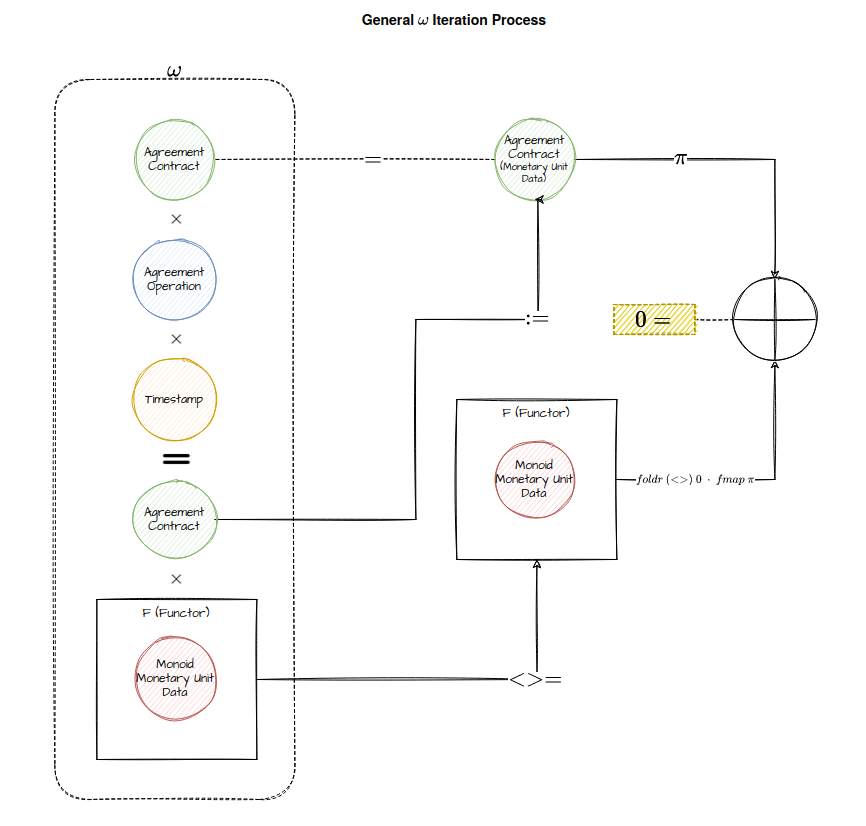
\includegraphics[width=1\textwidth]{../assets/agreement-contract-omega-function.png}
    \caption{Agreement Contract $\omega$ Function}
    \label{fig:ac-omega}
\end{figure}

It also illustrates that it is expected the process should respect the \textit{law of conservation
of value} mandated by the \textit{restricted money distribution} model.

It is also important to note that \textit{AgreementContract} itself is also
a \textit{MonetaryUnitDataClass}, but it is not a semigroup, hence it is used to replace the
previous agreement contract data. This has optimization implications, as in that if agreement
contracts do not produce zero balance then they must be included in the $\nu$ function, that can
make the $\nu$ function $O(N)$ to the number of agreement contracts a monetary unit is
associated with.

It may have been self evident that agreement contract is a analogy to the fact that it encodes
``ongoing relationships'' like legal contracts do between bearers.

\section{Lens Data Accessors}

In order to support \textit{index abstraction} in the denotational payment primitives, Monetary unit
data are created with \textit{lens data accessors}\footfullcite{clarke2020profunctor}:

\begin{code}
-- representation of lenses
data Lens a b s t = Lens { view :: s -> a, update :: (b, s) -> t }
-- the pro-functor version of it
type Lens s t a b = forall f. Functor f => (a -> f b) -> s -> f t
\end{code}

The pro-functor version of lens might seem very obscure at first, but its data representation is
rather self-explanatory: a lens is simply a pair of getter ($view$) and setter ($update$) encoded in
the data.

With the help of Lens, then we can create the payment primitives independent of the choices between
1-to-1, 1-to-N, etc. Here are how they are defined for each class of payment primitives:

\section{Useful Agreements}

\subsection{Instant Value MUD}

This is for agreements where value is instantly transferred.

\begin{code}
class ( Default amuLs
      , SuperfluidSystemTypes sft
      ) => MonetaryUnitLenses amuLs sft | amuLs -> sft where
    untappedValue :: Lens' amuLs (UntappedValue (SFT_MVAL sft))

type MonetaryUnitData :: Type -> Type -> Type
newtype MonetaryUnitData amuLs sft =
    MkMonetaryUnitData { getMonetaryUnitLenses :: amuLs }
    deriving (Default)

instance MonetaryUnitLenses amuLs sft
    => Semigroup (MonetaryUnitData amuLs sft) where
    MkMonetaryUnitData a <> MkMonetaryUnitData b =
        let c = a & over untappedValue (+ b^.untappedValue)
        in MkMonetaryUnitData c

instance MonetaryUnitLenses amuLs sft
    => MonetaryUnitDataClass (MonetaryUnitData amuLs sft) sft where
    balanceProvided (MkMonetaryUnitData a) _ =
        typedValuesToRTB [mkAnyTypedValue $ a^.untappedValue]
\end{code}

Note that (a) lens \textbf{operator (\string^.)} is the view function (getter) of data, (b)
semigroup \textbf{operator ($<>$)} defines how two monetary unit data can be combined into one.

\subsection{Constant Flow Agreement (CFA) MUD}

A more interesting case is where monetary value is changing continuously over time at a constant
rate:

\begin{code}
class ( Default amuLs
      , SuperfluidSystemTypes sft
      ) => MonetaryUnitLenses amuLs sft | amuLs -> sft where
    settledAt    :: Lens' amuLs (SFT_TS sft)
    settledValue :: Lens' amuLs (UntappedValue (SFT_MVAL sft))
    netFlowRate  :: Lens' amuLs (SFT_MVAL sft)

type MonetaryUnitData :: Type -> Type -> Type
newtype MonetaryUnitData amuLs sft =
    MkMonetaryUnitData { getMonetaryUnitLenses :: amuLs }
    deriving (Default)

instance MonetaryUnitLenses amuLs sft
    => Semigroup (MonetaryUnitData amuLs sft) where
    MkMonetaryUnitData a <> MkMonetaryUnitData b =
        let t  = a^.settledAt
            t' = b^.settledAt
            settledΔ = MkUntappedValue $ a^.netFlowRate * fromIntegral (t' - t)
            c = a & set  settledAt    t'
                  & over netFlowRate  (+ b^.netFlowRate)
                  & over settledValue (+ (b^.settledValue + settledΔ))
        in MkMonetaryUnitData c

instance MonetaryUnitLenses amuLs sft
    => MonetaryUnitDataClass (MonetaryUnitData amuLs sft) sft where
    balanceProvided (MkMonetaryUnitData a) t =
        let b = uval_s + coerce (fr * fromIntegral (t - t_s))
        in  typedValuesToRTB [ mkAnyTypedValue b ]
        where t_s    = a^.settledAt
              uval_s = a^.settledValue
              fr     = a^.netFlowRate
\end{code}

Note the implementation of semigroup binary operator, this is where the optimization occurs: to use
$netFlowRate$ to fold monetary unit data into a single value.

\subsection{Decaying Flow Agreement (CFA) MUD}

\begin{code}
class ( Default amuLs
      , SuperfluidSystemTypes sft
      ) => MonetaryUnitLenses amuLs sft | amuLs -> sft where
    decayingFactor  :: Lens' amuLs (SFT_FLOAT sft)
    settledAt       :: Lens' amuLs (SFT_TS sft)
    αVal            :: Lens' amuLs (SFT_FLOAT sft)
    εVal            :: Lens' amuLs (SFT_FLOAT sft)

type MonetaryUnitData :: Type -> Type -> Type
newtype MonetaryUnitData amuLs sft =
    MkMonetaryUnitData { getMonetaryUnitLenses :: amuLs }
    deriving (Default)

instance MonetaryUnitLenses amuLs sft
    => Semigroup (MonetaryUnitData amuLs sft) where
    MkMonetaryUnitData a <> MkMonetaryUnitData b =
        let c = a & set  settledAt     (b^.settledAt)
                  & over αVal          (\α -> α * exp (-λ * t_Δ) - ε')
                  & over εVal          (+ ε')
        in MkMonetaryUnitData c
        where ε'  = b^.εVal
              λ   = b^.decayingFactor
              t_Δ = fromIntegral (b^.settledAt - a^.settledAt)

instance MonetaryUnitLenses amuLs sft
    => MonetaryUnitDataClass (MonetaryUnitData amuLs sft) sft where
    balanceProvided (MkMonetaryUnitData a) t =
        let b = ceiling $ α * exp (-λ * t_Δ) + ε
        in  typedValuesToRTB [ (mkAnyTypedValue . MkUntappedValue) b ]
        where t_s   = a^.settledAt
              α     = a^.αVal
              ε     = a^.εVal
              λ     = a^.decayingFactor
              t_Δ   = fromIntegral (t - t_s)
\end{code}

\subsection{Universal Index (UIDX)}

An universal index then can be implemented trivially by representing lenses using the record syntax
directly. For example, for constant flow monetary unit data:

\begin{code}
data MonetaryUnitLenses sft = MonetaryUnitLenses
    { settled_at    :: SFT_TS sft
    , settled_value :: UntappedValue (SFT_MVAL sft)
    , net_flow_rate :: SFT_MVAL sft
    } deriving (Generic)

deriving instance SuperfluidSystemTypes sft
    => Default (MonetaryUnitLenses sft)

-- | Monetary unit lenses for the universal index.
instance SuperfluidSystemTypes sft
    => CFMUD.MonetaryUnitLenses (MonetaryUnitLenses sft) sft where
    settledAt          = $(field 'settled_at)
    settledValue       = $(field 'settled_value)
    netFlowRate        = $(field 'net_flow_rate)
\end{code}

The $field$ is a template Haskell function to generate lens from record fields.

\subsection{Proportional Distribution Index (PDIDX)}

Proportional distribution index describes on-going \textit{subscription} agreement contracts between
one \textit{publisher} and many \textit{subscribers} to the publisher's \textit{distribution}.

Its instant value variance is called \textit{``Instant Distribution Agreement (IDA)''}.

Its constant flow variance is called \textit{``Constant Flow Distribution Agreement (CFDA)''}.

\section{Hierarchy of Agreements}

To finish, figure \ref{fig:ac-agreement-data-structures} is the illustration of data structures for
the denotational payment primitives implemented with agreement framework.

\begin{figure}[H]
    \centering
    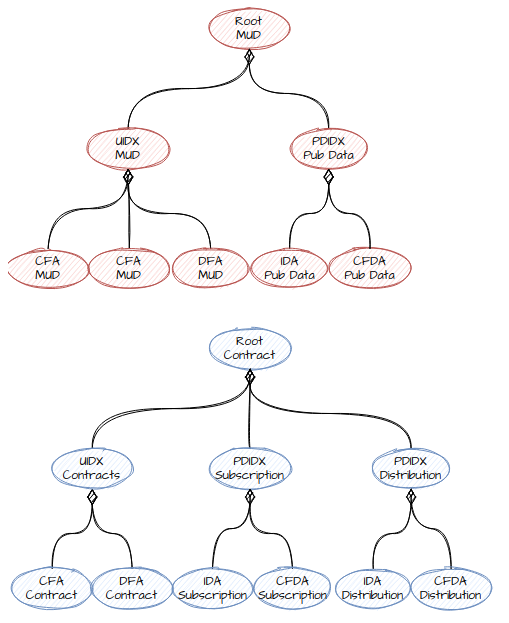
\includegraphics[width=0.9\textwidth]{../assets/agreement-data-structures.png}
    \caption{Agreement Data Structures}
    \label{fig:ac-agreement-data-structures}
\end{figure}

Note that with \textit{Root MUD}, any monetary unit can traverse all its MUDs; and with \textit{Root
Contract} relations between monetary units can also be searched by a simple algorithm.

This concludes the overview of the Superfluid protocol implementation. For more details, one should
refer to the code repository mentioned before.

%%%%%%%%%%%%%%%%%%%%%%%%%%%%%%%%%%%%%%%%%%%%%%%%%%%%%%%%%%%%%%%%%%%%%%%%%%%%%%%%%%%%%%%%%%%%%%%%%%%%
\part{Notes on Future Investigations}
%%%%%%%%%%%%%%%%%%%%%%%%%%%%%%%%%%%%%%%%%%%%%%%%%%%%%%%%%%%%%%%%%%%%%%%%%%%%%%%%%%%%%%%%%%%%%%%%%%%%

\section{Restatement in Agda, Correctness and Equivalence Proofs}

One of the advantages of using Haskell language to write the reference implementation was its
industrial strength. Because of that, the implementation could be easily integrated into a
production code base without significant performance compromises.

However, one major disadvantage is that it is not equipped with sufficient apparatus for program
correctness proofs. The best it can offer without using more experimental Haskell features is to
use \textit{QuickCheck}\footnote{\url{https://wiki.haskell.org/QuickCheck} - Haskell wiki page for
QuickCheck.} to test the necessary laws are not violated using randomized test vector.

To amend this deficiency, \textit{Agda programming language} comes as a great candidate for a
different constructive restatement of the formal specification.

It is based on the insight of the deep connection (equivalence/isomorphism) between logic and
dependently typed programming, often called "the Curry–Howard correspondence", as discovered and
developed during the 20th century (explained in \cite{wadler2015propositions} by Phillip Wadler as
``Propositions as Types''). Agda being a dependently typed functional programming language fully
embodies this insight, hence a good candidate for creating provable correct program.

To learn more about Agda, refer to these footnotes
\footnote{\url{https://plfa.github.io/} - Programming Language Foundations in Agda.}
\footnote{\url{https://wiki.portal.chalmers.se/agda/pmwiki.php} - Agda Wiki.}
\footnote{\url{https://wiki.portal.chalmers.se/agda/Main/Community} - Agda community page.}.

\section{Future Papers on Modern Payment System}

The next yellow paper will formalize how the denotational payment primitives can be stitched
together using a powerful combinator library pattern briefly described
in \cite{peyton2000composing}.

The execution environments for these financial contracts are also fertile ground for new ideas, from
deterministic execution avoiding the usage of buffer, to using distributed ledger technology to
deep-embed these financial contracts in the consensus layer.

\section{General Accounting Domains \& Real Time Finance}

\begin{displayquote}
Accounting, also known as accountancy, is the measurement, processing, and communication of
financial and non financial information about economic entities such as businesses and
corporations. \footfullcite{needles2013principles}
\end{displayquote}

The \textit{real time balance} introduced in this paper can be seen as a instance in
the \textit{general accounting domain} specifically for financial contracts in dealing with payment
primitives, which can be seen as a real time version of the cash flow accounting. Along with balance
sheet accounting, income statement accounting, the conversion between these instances of general
accounting domains are often called ``reconciliations''.

More work can be done on how to create a simple and elegant automation system for the
reconciliations.

\paragraph{Real Time Finance}

\emph{
We define the term \textbf{real time finance} to mean a financial system where its payment system is
modernized to handle money distribution continuously over time, its financial contracts are
compositional, and its general accounting domain are automated and processed in real time.  }

%%%%%%%%%%%%%%%%%%%%%%%%%%%%%%%%%%%%%%%%%%%%%%%%%%%%%%%%%%%%%%%%%%%%%%%%%%%%%%%%%%%%%%%%%%%%%%%%%%%%
\part*{Conclusions}
%%%%%%%%%%%%%%%%%%%%%%%%%%%%%%%%%%%%%%%%%%%%%%%%%%%%%%%%%%%%%%%%%%%%%%%%%%%%%%%%%%%%%%%%%%%%%%%%%%%%

This paper defines the what constitutes a modern payment system, with its payment primitives
formally specified using denotational semantics and restated using Haskell programming
language. Along with a reference implementation of the specification, we want to make a case that
marrying with the progress of computer science, the way of money performing its function of medium
of exchange can have a modern upgrade.

Absent of any claim on whether if such modern upgrade is needed, we invite the readers to ask
ourselves a question together: with electronic money increasingly being used, should we keep
emulating the function money of its traditional quality, or could we rethink what it may be in the
information age?

In future work, we will look into deeper other topics of real time finance, and continue to refine
the methodology used to achieve \textit{simple and precise} specifications guiding correct and
efficient engineering.

%%%%%%%%%%%%%%%%%%%%%%%%%%%%%%%%%%%%%%%%%%%%%%%%%%%%%%%%%%%%%%%%%%%%%%%%%%%%%%%%%%%%%%%%%%%%%%%%%%%%
\newpage
\printbibliography{}
%%%%%%%%%%%%%%%%%%%%%%%%%%%%%%%%%%%%%%%%%%%%%%%%%%%%%%%%%%%%%%%%%%%%%%%%%%%%%%%%%%%%%%%%%%%%%%%%%%%%

\end{document}
